% !TEX root =../main.tex

\chapter{Beispiel}

Hier etwas Text zur Einleitung. Ye ist meine absolute Lieblings Ye.

\section{Ziel der Arbeit}

Ja, wir finden auch, dass man über die Copy noch mal reden sollte. Das hier kann es jedenfalls nicht sein. Das klingt ja wie auf dem Totenbett getextet. Da muss wesentlich mehr Produktaussage rein. Ja, wir finden auch, dass man über die Copy noch mal reden sollte. Das hier kann es jedenfalls nicht sein. Das klingt ja wie auf dem Totenbett getextet. Da muss wesentlich mehr Produktaussage rein. Ja, wir finden auch, dass man über die Copy noch mal reden sollte.

\subsection{Motivation}

Ja, wir finden auch, dass man über die Copy noch mal reden sollte. Das hier kann es jedenfalls nicht sein. Das klingt ja wie auf dem Totenbett getextet. Da muss wesentlich mehr Produktaussage rein. Ja, wir finden auch, dass man über die Copy noch mal reden sollte. Das hier kann es jedenfalls nicht sein. Das klingt ja wie auf dem Totenbett getextet. Da muss wesentlich mehr Produktaussage rein. Ja, wir finden auch, dass man über die Copy noch mal reden sollte.

\subsubsection{Meine Motivation}

Ja, wir finden auch, dass man über die Copy noch mal reden sollte. Das hier kann es jedenfalls nicht sein. Das klingt ja wie auf dem Totenbett getextet. Da muss wesentlich mehr Produktaussage rein. Ja, wir finden auch, dass man über die Copy noch mal reden sollte. Das hier kann es jedenfalls nicht sein. Das klingt ja wie auf dem Totenbett getextet. Da muss wesentlich mehr Produktaussage rein. Ja, wir finden auch, dass man über die Copy noch mal reden sollte.

\paragraph{Ein Paragraph}

Ja, wir finden auch, dass man über die Copy noch mal reden sollte. Das hier kann es jedenfalls nicht sein. Das klingt ja wie auf dem Totenbett getextet. Da muss wesentlich mehr Produktaussage rein. Ja, wir finden auch, dass man über die Copy noch mal reden sollte. Das hier kann es jedenfalls nicht sein. Das klingt ja wie auf dem Totenbett getextet. Da muss wesentlich mehr Produktaussage rein. Ja, wir finden auch, dass man über die Copy noch mal reden sollte.

\subparagraph{Ein Unterparagraph}

Ja, wir finden auch, dass man über die Copy noch mal reden sollte. Das hier kann es jedenfalls nicht sein. Das klingt ja wie auf dem Totenbett getextet. Da muss wesentlich mehr Produktaussage rein. Ja, wir finden auch, dass man über die Copy noch mal reden sollte. Das hier kann es jedenfalls nicht sein. Das klingt ja wie auf dem Totenbett getextet. Da muss wesentlich mehr Produktaussage rein. Ja, wir finden auch, dass man über die Copy noch mal reden sollte.

\section{Textauszeichnung (logisches Markup)}

Es können beliebig viele Befehle definiert werden, um Text besonders hervorzuheben. Zwei vordefinierte Befehle stehen bereits zur Verfügung. Ein Befehl für generelles hervorheben von Text und ein Befehl, um Quellcode-Begriffe hervorzuheben. Falls weitere Typen der Textauszeichnung gewünscht sind, können diese einfach hinzugefügt werden.

\emph{Hervorgehobener Text}

\code{Begriffe aus dem Quellcode}

\section{Aufzählungen}

Aufzählung mit Stichpunkten:

\begin{itemize}
	\item Erster Punkt
	\item Zweiter Punkt
	\item Dritter Punkt
\end{itemize}

Nummerierte Aufzählung.

\begin{enumerate}
	\item Erster Punkt
	\item Zweiter Punkt
	\item Dritter Punkt
\end{enumerate}

\section{Abbildungen}

In der Abbildung \vref{fig:wursthund} ist der so genannte Wursthund in seiner natürlichen Umgebung zu sehen.

\begin{figure}[htbp]
	\centering
	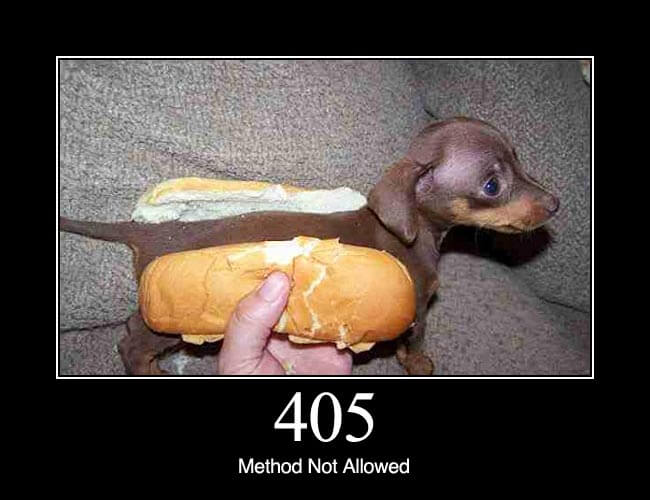
\includegraphics[width=10cm]{bilder/wursthund.jpg}
	\caption{Wursthund}
	\label{fig:wursthund}
\end{figure}

\section{Tabellen}

Ein Beispiel für eine Tabelle, mit variabler Spaltenbreite, ist durch Tabelle \vref{tab:variable-breite} dargestellt.

\begin{table}[htbp]
\centering
\begin{tabular}{l l l}
\toprule
Ziel            & Abfahrt      & Dauer \\
\midrule
Frankfurt       & stündlich    & 3:20 \\
Berlin          & stündlich    & 5:40 \\
Hamburg         & alle 5\,h    & 5:20 \\
\bottomrule
\end{tabular}
\caption{Tabelle mit variabler Spaltenbreite}
\label{tab:variable-breite}
\end{table}

Ein Beispiel für eine Tabelle, mit fester Spaltenbreite, ist durch Tabelle \vref{tab:feste-breite} dargestellt.

\begin{table}[htbp]
\centering
\begin{tabular}{p{3.5cm} p{5.5cm}}
\toprule
\textbf{Spalte 1}  & \textbf{Spalte 2}\\
\midrule
\textbf{Eintrag 1} & \textbf{Eintrag 2}\\
Daten              & Daten\\
Daten              & Daten\\
Daten              & Daten\\
\midrule
\textbf{Eintrag 1} & \textbf{Eintrag 2}\\
Daten              & Daten\\
Daten              & Daten\\
Daten              & Daten\\
\bottomrule
\end{tabular}
\caption{Tabelle mit fester Spaltenbreite}
\label{tab:feste-breite}
\end{table}

Eine lange Tabelle, welche sich über mehrere Seiten erstrecken kann ist in Tabelle \ref{tab:lange-tabelle} dargestellt.

\begin{longtable}{p{2cm} p{2cm} p{2cm} p{2cm} p{2cm}}
\toprule
\textbf{\O min}& \textbf{\O max}& \textbf{Wert 1}& \textbf{Wert 2}& \textbf{Wert 3}\\
\midrule
 6& 10&  56& 100& 20,00\\
 6& 10& 100& 150& 20,00\\
 6& 10& 150& 200& 20,00\\
 6& 10& 200& 250& 20,00\\
 6& 10& 250& 300& 20,00\\
 6& 10& 300& 350& 20,00\\
 6& 10& 350& 400& 20,00\\
10& 14&  63& 100& 20,00\\
10& 14& 100& 150& 20,00\\
10& 14& 150& 200& 20,00\\
10& 14& 200& 250& 20,00\\
10& 14& 250& 300& 20,00\\
10& 14& 300& 350& 20,00\\
10& 14& 350& 400& 20,00\\
\bottomrule
\caption{Lange Tabelle}
\label{tab:lange-tabelle}
\end{longtable}

\section{Verweise}

Es existieren mehrere Arten auf Objekte zu verweisen.

Abbildungsnummer: \ref{fig:wursthund}

Abbildungsnummer und relative Seitenzahl: \vref{fig:wursthund}

Seitenzahl: \pageref{fig:wursthund}

Relative Seitenzahl: \vpageref{fig:wursthund}

\section{Beschreibungsumgebung}

\begin{description}
\item[Begriff Nummer 1] Ja, wir finden auch, dass man über die Copy noch mal reden sollte. Das hier kann es jedenfalls nicht sein. Das klingt ja wie auf dem Totenbett getextet. Da muss wesentlich mehr Produktaussage rein. Ja, wir finden auch, dass man über die Copy noch mal reden sollte. Das hier kann es jedenfalls nicht sein. Das klingt ja wie auf dem Totenbett getextet. Da muss wesentlich mehr Produktaussage rein. Ja, wir finden auch, dass man über die Copy noch mal reden sollte.
\item[Begriff Nummer 2] Ja, wir finden auch, dass man über die Copy noch mal reden sollte. Das hier kann es jedenfalls nicht sein. Das klingt ja wie auf dem Totenbett getextet. Da muss wesentlich mehr Produktaussage rein. Ja, wir finden auch, dass man über die Copy noch mal reden sollte. Das hier kann es jedenfalls nicht sein. Das klingt ja wie auf dem Totenbett getextet. Da muss wesentlich mehr Produktaussage rein. Ja, wir finden auch, dass man über die Copy noch mal reden sollte.
\end{description}

\section{Fußnoten}

Zu diesem Satz existiert eine Fußnote. Sieh nach, ob du sie finden kannst.\footnote{Großartig! Du hast sie gefunden.}

\section{Quellenangabe}

Ja, wir finden auch, dass man über die Copy noch mal reden sollte. Das hier kann es jedenfalls nicht sein. Das klingt ja wie auf dem Totenbett getextet. Da muss wesentlich mehr Produktaussage rein. Ja, wir finden auch, dass man über die Copy noch mal reden sollte. Das hier kann es jedenfalls nicht sein. Das klingt ja wie auf dem Totenbett getextet. Da muss wesentlich mehr Produktaussage rein. Ja, wir finden auch, dass man über die Copy noch mal reden sollte. \cite{angenendt}

\section{Quellcode}